\documentclass{article}
\usepackage{graphicx}
\usepackage{hyperref}
\graphicspath{{./figs/}}{}
\usepackage{listings}
\title{
HLS-Assignment 7
}
\begin{document}
\maketitle
\hfill \textbf{Sampath Govardhan} \\
\null \hfill \textbf{FWC22071}\\

\section{Problem Statement}
\begin{lstlisting}
Implement a module in HLS that models a basic FIR filter as specified on this 
web page: https://sestevenson.wordpress.com/implementation-of-fir-filtering-in-c
part-1/. The web page also has C code which you should use as reference for your
HLS design. Your task is to model the design in the most efficient manner 
possible for the hardware (e.g. small clock period, lower initiation interval, 
less resource consumption, etc.). After designing, you should compare your output
against the reference output generated by the C code for the same set of input
vectors, using a self checking testbench that allows for a 5% difference in 
output values generated by the C code and the HLS code. Use at least two 
different input vectors. Also, the  HLS design should use appropriate fixed 
point format instead of floating point format wherever applicable. The C code 
from the website can be integrated as part of your HLS testbench if you name 
both the design modules differently, for e.g., firFloat for C module and 
firFixed for HLS module. This will enable you to pass the input vectors to both 
the modules and compare the outputs, in a single testbench.
\end{lstlisting}
\vspace{3cm}
\section{Header File}
\begin{lstlisting}
#ifndef FIR_H_
#define FIR_H_
#define N 4
#include "ap_fixed.h"
#include <string.h>
#include <math.h>
#include <iostream>
#include <fstream>

using namespace std;


typedef ap_fixed<24,12> in;
typedef ap_fixed<48,24> out;

void fir (out *y, in c[N], in x);
void firFloatInit( void );
void intToFloat( int *input, double *output, int length );
void firFloat( double *coeffs, double *input, double *output, int length, int
filterLength );
void floatToInt( double *input, int *output, int length );

#endif

\end{lstlisting}
\vspace{5cm}
\section{firFixed.cpp Code}
\begin{lstlisting}
#include "fir.h"

void fir (out *y, in c[N], in x) {
#pragma HLS INTERFACE ap_none port=y
#pragma HLS INTERFACE ap_none port=c
#pragma HLS INTERFACE ap_none port=x


  static in shift_reg[N]={0};
#pragma HLS ARRAY_PARTITION variable=shift_reg complete dim=1
  out acc=0;
  in input_data=x;
  for (int i=N-1;i>=0;i--) {
#pragma HLS PIPELINE
	  in current_data;
	if (i==0) {
		 current_data = input_data;
			shift_reg[0]=input_data;
    } else {
        current_data = shift_reg[i-1];
        shift_reg[i] = current_data;

    }
    acc+=current_data*c[i];;
  }
  *y=acc;
}

\end{lstlisting}
\vspace{5cm}
\section{FirFloat.cpp Code}
\begin{lstlisting}
#include "fir.h"
//////////////////////////////////////////////////////////////
// Filter Code Definitions
//////////////////////////////////////////////////////////////
// maximum number of inputs that can be handled
// in one function call
#define MAX_INPUT_LEN 10
// maximum length of filter than can be handled
#define MAX_FLT_LEN 10
// buffer to hold all of the input samples
#define BUFFER_LEN (MAX_FLT_LEN - 1 + MAX_INPUT_LEN)
// array to hold input samples
double insamp[ BUFFER_LEN ];
// FIR init
void firFloatInit( void )
{
 memset( insamp, 0, sizeof( insamp ) );
}

void intToFloat( int *input, double *output, int length )
{
 int i;
 for ( i = 0; i < length; i++ ) {
 output[i] = (double)input[i];
 }
}

// the FIR filter function
void firFloat( double *coeffs, double *input, double *output,
 int length, int filterLength )
{
 double acc; // accumulator for MACs
 double *coeffp; // pointer to coefficients
 double *inputp; // pointer to input samples
 int n;
 int k;
 // put the new samples at the high end of the buffer
 memcpy( &insamp[filterLength - 1], input,
 length * sizeof(double) );
 // apply the filter to each input sample
 for ( n = 0; n < length; n++ ) {
 // calculate output n
 coeffp = coeffs;
 inputp = &insamp[filterLength - 1 + n];
 acc = 0;
 for ( k = 0; k < filterLength; k++ ) {
 acc += (*coeffp++) * (*inputp--);
 }
 output[n] = acc;
 }
 // shift input samples back in time for next time
 memmove( &insamp[0], &insamp[length],
 (filterLength - 1) * sizeof(double) );
}
void floatToInt( double *input, int *output, int length )
{
 int i;
 for ( i = 0; i < length; i++ ) {
 // add rounding constant
 input[i] += 0.5;
 // bound the values to 16 bits
 if ( input[i] > 32767.0 ) {
 input[i] = 32767.0;
 } else if ( input[i] < -32768.0 ) {
 input[i] = -32768.0;
 }
 // convert
 output[i] = (int)input[i];
 }
}

\end{lstlisting}
\vspace{3cm}

\section{Test Bench Code}
\begin{lstlisting}
#include "fir.h"
#define SAMPLES 5

int main()
{

  int input[SAMPLES];  //fir float
  in input1[SAMPLES];  //fir fixed

  double coeffs[ N ];  //fir float
  in taps[ N ];        //fir fixed

  int output[SAMPLES];           //fir float
  out output1[SAMPLES];          //fir fixed

 double floatInput[SAMPLES];
 double floatOutput[SAMPLES];

 ifstream inputFile("inp.dat");
 ifstream inputFile1("inp.dat");
 ifstream inputFile2("coef.dat");
 ifstream inputFile3("coef.dat");
 ofstream outputfile("out.dat");

for (int p=1;p<3;p++){

        for (int j = 0; j < SAMPLES; j++) {
            inputFile >> input[j];
        }

         for (int j = 0; j < SAMPLES; j++) {
             inputFile1 >> input1[j];
         }

         for (int j = 0; j < N; j++) {
             inputFile2 >> coeffs[j];
         }

          for (int j = 0; j < N; j++) {
              inputFile3 >> taps[j];
          }


 // initialize the filter
 firFloatInit();
 // process all of the samples
 // convert to doubles
    intToFloat( input, floatInput,SAMPLES);
 // perform the filtering with C Code
    firFloat( coeffs, floatInput, floatOutput, SAMPLES , N );
 // convert to int
    floatToInt( floatOutput, output, SAMPLES);
    int sum1=0;
    out sum2=0;
   for (int j=0;j<SAMPLES;j++){
// perform the filtering with HLS code
	 fir(&output1[j],taps,input1[j]);

	 sum1+=output[j];
	 sum2+=output1[j];
 }

	 if (abs(sum1- double(sum2))/double(sum2) > 0.05){
	       cout << "TEST CASE " <<p<<" DID NOT PASSED AS DIFFERENCE IS MORE
	       THAN 5% " << endl;
	 }
	    else{
	       cout << "TEST CASE "<<p<<" PASSED " << endl;
	    }
      outputfile<<"TEST CASE :"<<p<<" "<<"(HLS ~= C)"<<endl;
	  outputfile<<"     "<<endl;
	  for (int j = 0; j < SAMPLES; j++) {
	     outputfile << output1[j]<<"  ~=  "<< output[j]<< endl;
	   }
	  outputfile<<" "<<endl;

}
 inputFile.close();
 inputFile1.close();
 inputFile2.close();
 inputFile3.close();
 outputfile.close();
 return 0;
}



\end{lstlisting}
\vspace{3cm}

\section{inp.dat file}
\begin{lstlisting}
1 2 3 4 5
5 4 3 2 1


\end{lstlisting}
\vspace{3cm}
\section{coef.dat file}
\begin{lstlisting}
2 3 4 1 
0.2 0.3 0.4 0.1


\end{lstlisting}
\vspace{3cm}
\section{out.dat file}
\begin{lstlisting}
TEST CASE :1 (HLS ~= C)
     
2  ~=  2
7  ~=  7
16  ~=  16
26  ~=  26
36  ~=  36
 
TEST CASE :2 (HLS ~= C)
     
4.39795  ~=  1
4.69775  ~=  2
4.29785  ~=  4
3.39819  ~=  3
2.39868  ~=  2


\end{lstlisting}
\vspace{3cm}
\section{C simulation Output}
\begin{lstlisting}
INFO: [SIM 2] *************** CSIM start ***************
INFO: [SIM 4] CSIM will launch GCC as the compiler.
   Compiling ../../../../firFloat.cpp in debug mode
   Compiling ../../../../firTB.cpp in debug mode
   Compiling ../../../../firFixed.cpp in debug mode
   Generating csim.exe
TEST CASE 1 PASSED 
TEST CASE 2 DID NOT PASSED AS DIFFERENCE IS MORE THAN 5% 
INFO: [SIM 1] CSim done with 0 errors.
INFO: [SIM 3] *************** CSIM finish ***************



\end{lstlisting}
\vspace{3cm}
\vspace{15cm}


\section{HLS Resource Consumption}
\vspace{3cm}
\begin{figure}[h]
    \centering
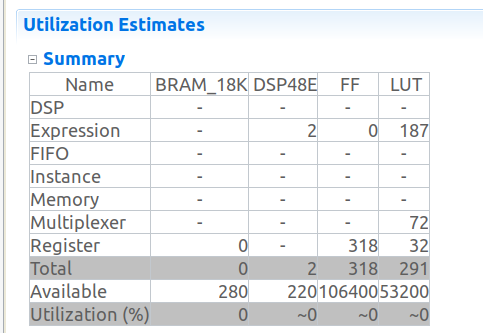
\includegraphics[width=\columnwidth]{1.png}
    \caption{Resource Consumption}
    \label{fig:my_label}
\end{figure}

\vspace{5cm}


\section{HLS Timing Report}
\vspace{1cm}
\begin{figure}[h]
    \centering
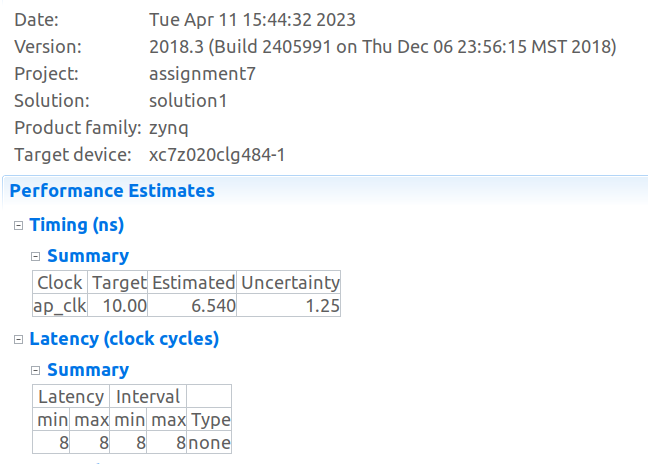
\includegraphics[width=\columnwidth]{figs/2.png}
    \caption{Timing Report}
    \label{fig:my_label}
\end{figure}

\vspace{10cm}


\section{Interfaces Report}
\vspace{1cm}
\begin{figure}[h]
    \centering
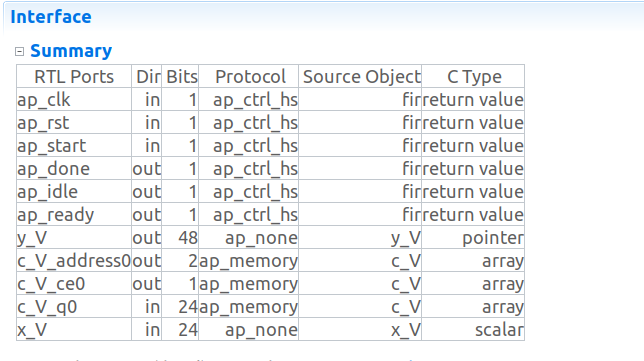
\includegraphics[width=\columnwidth]{figs/3.png}
    \caption{Interface Summmary}
    \label{fig:my_label}
\end{figure}
\vspace{5cm}

\section{C/RTL Cosimulation Output}
\begin{lstlisting}
Starting C/RTL cosimulation ...
/tools/Xilinx/Vivado/2018.3/bin/vivado_hls /home/sam-admin/git/Training/HLS_Assignments/A7/codes/assignment7/solution1/cosim.tcl
INFO: [HLS 200-10] Running '/tools/Xilinx/Vivado/2018.3/bin/unwrapped/lnx64.o/vivado_hls'
INFO: [HLS 200-10] For user 'sam-admin' on host 'sampaths-lappie' (Linux_x86_64 version 5.19.0-38-generic) on Tue Apr 11 15:45:49 IST 2023
INFO: [HLS 200-10] On os Ubuntu 22.04.2 LTS
INFO: [HLS 200-10] In directory '/home/sam-admin/git/Training/HLS_Assignments/A7/codes'
INFO: [HLS 200-10] Opening project '/home/sam-admin/git/Training/HLS_Assignments/A7/codes/assignment7'.
INFO: [HLS 200-10] Opening solution '/home/sam-admin/git/Training/HLS_Assignments/A7/codes/assignment7/solution1'.
INFO: [SYN 201-201] Setting up clock 'default' with a period of 10ns.
INFO: [HLS 200-10] Setting target device to 'xc7z020clg484-1'
INFO: [COSIM 212-47] Using XSIM for RTL simulation.
INFO: [COSIM 212-14] Instrumenting C test bench ...
   Build using "/tools/Xilinx/Vivado/2018.3/tps/lnx64/gcc-6.2.0/bin/g++"
   Compiling apatb_fir.cpp
   Compiling firFixed.cpp_pre.cpp.tb.cpp
   Compiling firFloat.cpp_pre.cpp.tb.cpp
   Compiling firTB.cpp_pre.cpp.tb.cpp
   Generating cosim.tv.exe
INFO: [COSIM 212-302] Starting C TB testing ... 
TEST CASE 1 PASSED 
TEST CASE 2 DID NOT PASSED AS DIFFERENCE IS MORE THAN 5% 
INFO: [COSIM 212-333] Generating C post check test bench ...
INFO: [COSIM 212-12] Generating RTL test bench ...
INFO: [COSIM 212-323] Starting verilog simulation. 
INFO: [COSIM 212-15] Starting XSIM ...
INFO: [XSIM 43-3496] Using init file passed via -initfile option "/tools/Xilinx/Vivado/2018.3/data/xsim/ip/xsim_ip.ini".
Vivado Simulator 2018.3
Copyright 1986-1999, 2001-2018 Xilinx, Inc. All Rights Reserved.
Running: /tools/Xilinx/Vivado/2018.3/bin/unwrapped/lnx64.o/xelab xil_defaultlib.apatb_fir_top glbl -prj fir.prj -L smartconnect_v1_0 -L axi_protocol_checker_v1_1_12 -L axi_protocol_checker_v1_1_13 -L axis_protocol_checker_v1_1_11 -L axis_protocol_checker_v1_1_12 -L xil_defaultlib -L unisims_ver -L xpm --initfile /tools/Xilinx/Vivado/2018.3/data/xsim/ip/xsim_ip.ini --lib ieee_proposed=./ieee_proposed -s fir 
Multi-threading is on. Using 6 slave threads.
WARNING: [XSIM 43-3431] One or more environment variables have been detected which affect the operation of the C compiler. These are typically not set in standard installations and are not tested by Xilinx, however they may be appropriate for your system, so the flow will attempt to continue.  If errors occur, try running xelab with the "-mt off -v 1" switches to see more information from the C compiler. The following environment variables have been detected:
    LIBRARY_PATH
INFO: [VRFC 10-2263] Analyzing SystemVerilog file "/home/sam-admin/git/Training/HLS_Assignments/A7/codes/assignment7/solution1/sim/verilog/glbl.v" into library work
INFO: [VRFC 10-311] analyzing module glbl
INFO: [VRFC 10-2263] Analyzing SystemVerilog file "/home/sam-admin/git/Training/HLS_Assignments/A7/codes/assignment7/solution1/sim/verilog/fir.v" into library xil_defaultlib
INFO: [VRFC 10-311] analyzing module fir
INFO: [VRFC 10-2263] Analyzing SystemVerilog file "/home/sam-admin/git/Training/HLS_Assignments/A7/codes/assignment7/solution1/sim/verilog/fir.autotb.v" into library xil_defaultlib
INFO: [VRFC 10-311] analyzing module apatb_fir_top
INFO: [VRFC 10-2263] Analyzing SystemVerilog file "/home/sam-admin/git/Training/HLS_Assignments/A7/codes/assignment7/solution1/sim/verilog/AESL_automem_c_V.v" into library xil_defaultlib
INFO: [VRFC 10-311] analyzing module AESL_automem_c_V
Starting static elaboration
Completed static elaboration
Starting simulation data flow analysis
Completed simulation data flow analysis
Time Resolution for simulation is 1ps
Compiling module xil_defaultlib.fir
Compiling module xil_defaultlib.AESL_automem_c_V
Compiling module xil_defaultlib.apatb_fir_top
Compiling module work.glbl
Built simulation snapshot fir


****** Webtalk v2018.3 (64-bit)
  **** SW Build 2405991 on Thu Dec  6 23:36:41 MST 2018
  **** IP Build 2404404 on Fri Dec  7 01:43:56 MST 2018
    ** Copyright 1986-2018 Xilinx, Inc. All Rights Reserved.


source /home/sam-admin/git/Training/HLS_Assignments/A7/codes/assignment7/solution1/sim/verilog/xsim.dir/fir/webtalk/xsim_webtalk.tcl -notrace
INFO: [Common 17-206] Exiting Webtalk at Tue Apr 11 15:46:52 2023...


****** xsim v2018.3 (64-bit)
  **** SW Build 2405991 on Thu Dec  6 23:36:41 MST 2018
  **** IP Build 2404404 on Fri Dec  7 01:43:56 MST 2018
    ** Copyright 1986-2018 Xilinx, Inc. All Rights Reserved.


source xsim.dir/fir/xsim_script.tcl
# xsim {fir} -autoloadwcfg -tclbatch {fir.tcl}
Vivado Simulator 2018.3
Time resolution is 1 ps
source fir.tcl
## run all
////////////////////////////////////////////////////////////////////////////////////
// Inter-Transaction Progress: Completed Transaction / Total Transaction
// Intra-Transaction Progress: Measured Latency / Latency Estimation * 100%
//
// RTL Simulation : "Inter-Transaction Progress" ["Intra-Transaction Progress"] @ "Simulation Time"
////////////////////////////////////////////////////////////////////////////////////
// RTL Simulation : 0 / 10 [0.00%] @ "125000"
// RTL Simulation : 1 / 10 [100.00%] @ "225000"
// RTL Simulation : 2 / 10 [100.00%] @ "315000"
// RTL Simulation : 3 / 10 [100.00%] @ "405000"
// RTL Simulation : 4 / 10 [100.00%] @ "495000"
// RTL Simulation : 5 / 10 [100.00%] @ "585000"
// RTL Simulation : 6 / 10 [100.00%] @ "675000"
// RTL Simulation : 7 / 10 [100.00%] @ "765000"
// RTL Simulation : 8 / 10 [100.00%] @ "855000"
// RTL Simulation : 9 / 10 [100.00%] @ "945000"
// RTL Simulation : 10 / 10 [100.00%] @ "1035000"
////////////////////////////////////////////////////////////////////////////////////
$finish called at time : 1075 ns : File "/home/sam-admin/git/Training/HLS_Assignments/A7/codes/assignment7/solution1/sim/verilog/fir.autotb.v" Line 327
## quit
INFO: [Common 17-206] Exiting xsim at Tue Apr 11 15:47:03 2023...
INFO: [COSIM 212-316] Starting C post checking ...
TEST CASE 1 PASSED 
TEST CASE 2 DID NOT PASSED AS DIFFERENCE IS MORE THAN 5% 
INFO: [COSIM 212-1000] *** C/RTL co-simulation finished: PASS ***
Finished C/RTL cosimulation.


\end{lstlisting}

\section{C/RTL Cosimulation Report}
\vspace{1cm}
\begin{figure}[h]
    \centering
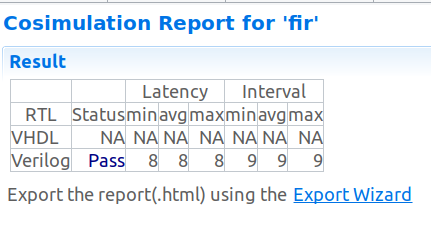
\includegraphics[width=\columnwidth]{figs/4.png}
    \caption{Cosimulation Report}
    \label{fig:my_label}
\end{figure}

\textbf{GITHUB :} \url{https://github.com/dk-425/Training.git}
\end{document}
